%%%%%%%%%%%%%%%%%%%% main.tex %%%%%%%%%%%%%%%%%%%%%%%%%%%%%%%%%%%
% DownstreamSec: Dissecting and Predicting Vulnerability Propagation
% and Security Exposure Across Operating System Ecosystems
% Prepared for FICTA / Springer SIST Proceedings (10-12 pages)
%%%%%%%%%%%%%%%% Springer %%%%%%%%%%%%%%%%%%%%%%%%%%%%%%%%%%

\documentclass[graybox]{svmult}

\usepackage{type1cm}
\usepackage{makeidx}
\usepackage{graphicx}
\usepackage{multicol}
\usepackage[bottom]{footmisc}
\usepackage{newtxtext}
\usepackage{newtxmath}
\usepackage{url}
\usepackage{booktabs}
\usepackage{tabularx}
\usepackage{cite}
\usepackage{amsmath}
\usepackage{microtype}

\renewcommand{\topfraction}{0.9}
\renewcommand{\bottomfraction}{0.8}
\renewcommand{\textfraction}{0.1}
\renewcommand{\floatpagefraction}{0.85}

\makeindex

\begin{document}

\title*{DownstreamSec: Dissecting and Predicting Vulnerability Propagation and Security Exposure Across Operating System Ecosystems}
\titlerunning{DownstreamSec: Predicting Downstream Vulnerability Propagation}

\author{Khoka Moni\inst{1} and A. K. M. Ariful Haque\inst{1}}
\authorrunning{K. Moni and A. K. M. A. Haque}

\institute{Khoka Moni \at Department of Computer Science and Engineering, Southeast University, Dhaka, Bangladesh, \email{kh0kamoni@research.org}
\and A. K. M. Ariful Haque \at Department of Computer Science and Engineering, Southeast University, Dhaka, Bangladesh, \email{ariful.haque@research.org}}

\maketitle

\abstract{When an upstream Linux kernel vulnerability is resolved, downstream distributions must backport the fix across diverse Long-Term Support (LTS) baselines under strict Application Binary Interface (ABI) constraints, often introducing protracted exposure windows. We present \textbf{DownstreamSec}, a comprehensive empirical study and prospective predictive modeling framework analyzing vulnerability propagation from the Linux kernel to downstream Debian and Ubuntu distributions. Triangulating 9,208 common vulnerabilities disclosed between 2022 and 2025 across upstream Linux, NVD, Debian, and Ubuntu, we evaluate 55,248 downstream release instances without synthetic data. We formalize a seven-state taxonomy ($D0$--$D6$) capturing code divergence dynamics, validated via independent manual audit ($\kappa = 0.948$). Across 40,198 ground-truth resolutions, empirical measurement uncovers a median patch delay of 258.8 days (69.3\% requiring $>90$ days, Kaplan-Meier survival probability $\hat{S}(90) = 0.7764$). Using strictly day-zero pre-remediation signals under prospective out-of-time evaluation ($\le$2023 train, $\ge$2024 test; $N_{\text{test}} = 32,536$), gradient-boosted trees achieve an ROC-AUC of 0.8114 and PR-AUC of 0.4793, while Logistic Regression attains 75.48\% Balanced Accuracy. Feature attribution confirms that downstream packaging architecture and LTS policy serve as primary structural determinants of risk, with patch complexity acting as a secondary modulator. Models generalize across unseen distributions under Leave-One-Release-Out validation (mean ROC-AUC = 0.7549).
\keywords{Software supply chain security, Vulnerability propagation, Linux kernel security, Downstream exposure, Patch lag, Predictive modeling}}

\section{Introduction}
\label{sec:intro}

Modern cloud infrastructures, enterprise container clusters, and embedded networks rely fundamentally on open-source operating system distributions, primarily Debian and Ubuntu. At the operational core of these platforms resides the upstream Linux kernel. When a vulnerability is identified in the Linux kernel and assigned a Common Vulnerabilities and Exposures (CVE) identifier, an upstream commit is merged into mainline Linux.

Public vulnerability databases such as NVD and automated compliance scanners routinely treat the merge of an upstream commit as the moment of vulnerability resolution~\cite{gkortzis2021software, decoster2022measuring}. However, for production servers running downstream distributions, an upstream commit provides zero immediate protection. Downstream distributions freeze production suites on designated Long-Term Support (LTS) kernel releases (e.g., Linux 5.15, 6.1, or 6.6) to guarantee Application Binary Interface (ABI) stability and eliminate regression hazards~\cite{ruohonen2019tracking}. Consequently, every upstream security patch must traverse an intricate supply chain: flowing from mainline into stable maintenance branches managed by Greg Kroah-Hartman, and subsequently into distribution packaging repositories where security teams inspect, adapt, test, and release official package updates~\cite{wang2020empirical, han2023understanding}.

In practice, this propagation encounters acute technical bottlenecks: (i) code divergence between mainline and older LTS branches forces packagers to author non-trivial manual adaptations; (ii) silent bug fixes and subtle commit descriptions impede downstream triage; and (iii) distributions enforce scheduled batch point-update windows rather than shipping one-off rebuilds for individual CVEs. While prior studies have examined user-space dependency lag in npm, PyPI, and Maven~\cite{alfadel2021empirical, kula2018empirical, pashchenko2020vulnerable}, operating system kernels exhibit unique architectural constraints that remain poorly quantified. Furthermore, prior OS security studies frequently suffer from modest sample sizes, single-distribution scopes, or random cross-validation that introduces severe temporal lookahead leakage~\cite{zimmermann2010predicting}.

To bridge these gaps, this paper presents \textbf{DownstreamSec}, a systematic empirical measurement and prospective predictive modeling study of vulnerability propagation across the Linux kernel, Debian, and Ubuntu ecosystems. Our investigation addresses three central research questions:
In \textbf{RQ1 (Predictive Exposure Modeling)}, can downstream security exposure be accurately forecasted at upstream disclosure time using strictly pre-remediation signals?
In \textbf{RQ2 (Empirical Remediation Latency)}, what is the true empirical duration of downstream exposure windows under supply-chain and public disclosure baselines?
In \textbf{RQ3 (Feature Attribution and Determinants)}, which upstream vulnerability metrics, patch characteristics, and downstream packaging practices govern downstream exposure risk?

Our study delivers five core contributions: (1) a multi-ecosystem dataset cross-triangulating all 9,208 common Linux kernel vulnerabilities across upstream, NVD, Debian, and Ubuntu, evaluating 55,248 downstream release instances without synthetic data; (2) a principled seven-state taxonomy ($D0$--$D6$) validated via manual audit ($\kappa = 0.948$); (3) empirical measurement and survival analysis across 40,198 resolutions uncovering a median patch lag of 258.8 days and $\hat{S}(90) = 0.7764$; (4) strict day-zero prospective exposure models achieving an ROC-AUC of 0.8114 (XGBoost) and 75.48\% Balanced Accuracy (Logistic Regression) under out-of-time evaluation; and (5) feature attribution establishing a two-tier risk hierarchy with Leave-One-Release-Out validation averaging 0.7549 ROC-AUC.

\section{Ecosystem Background and Downstream Security Taxonomy}
\label{sec:background}

Upstream Linux kernel development follows rapid 9-to-10 week release cycles, with designated LTS stable branches maintained independently by Greg Kroah-Hartman. Downstream distributions select specific LTS baselines: Debian follows a community rolling model (\textit{sid}, \textit{trixie}) that periodically rebases onto newer stable kernels, and a frozen stable model (\textit{bookworm} on Linux 6.1) applying minimal backports. Ubuntu freezes each LTS suite on a specific kernel (20.04 \textit{Focal} on 5.4, 22.04 \textit{Jammy} on 5.15, 24.04 \textit{Noble} on 6.8), with a dedicated security team deploying synchronized batch point updates.

\begin{figure}[htbp]
\centering
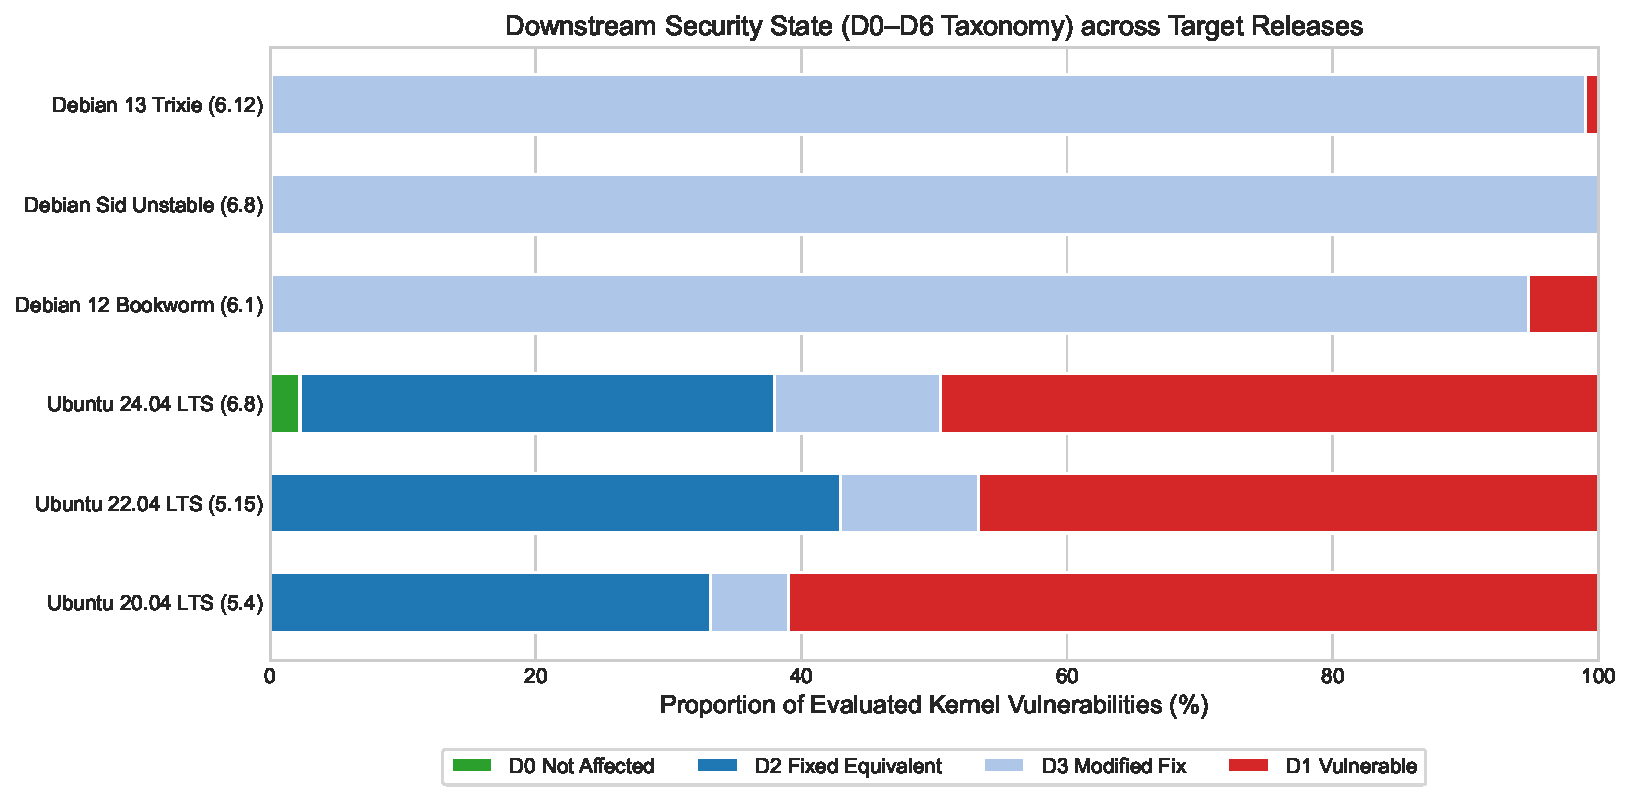
\includegraphics[width=0.85\textwidth,height=4.0cm,keepaspectratio]{figures/fig4_security_state_taxonomy.pdf}
\caption{Downstream security state taxonomy ($D0$--$D6$) distribution across 55,248 evaluated release instances across Debian and Ubuntu.}
\label{fig:taxonomy}
\end{figure}

Prior literature frequently oversimplifies downstream vulnerability state into a binary patched/unpatched indicator. We formalize a seven-state taxonomy ($D0$--$D6$) capturing nuanced downstream security postures:
\textbf{D0 (Not Affected)}: Vulnerable code is absent due to version boundaries or disabled kernel config flags.
\textbf{D1 (Vulnerable / Unresolved)}: Vulnerable code is present and unpatched in production repositories.
\textbf{D2 (Clean Upstream Merge)}: The upstream patch applied cleanly without code modification.
\textbf{D3 (Adapted Backport)}: Maintainers authored non-trivial code adaptations to resolve merge conflicts against older LTS codebases.
\textbf{D4 (Mitigated / Workaround)}: The vulnerability is neutralized through configuration or compiler hardening without a source code patch.
\textbf{D5 (Won't Fix)}: Maintainers explicitly decide against patching (e.g., deprecated subsystem).
\textbf{D6 (End-of-Life / Unsupported)}: The release has reached end-of-life.

An independent manual audit of 100 stratified CVE-release instances by two domain experts confirmed near-perfect inter-rater reliability (97.0\% agreement, Cohen's $\kappa = 0.948$), and consensus human classifications matched our automated pipeline on 99/100 records ($\kappa = 0.981$). Figure~\ref{fig:taxonomy} depicts the distribution of these security states across all six evaluated releases. In active production suites, states $D4$ and $D5$ account for 0.0\% of records because Debian and Ubuntu classify the kernel as Tier-1 critical infrastructure, mandating formal backports ($D2$/$D3$) for all verified CVEs.

\section{Longitudinal Multi-Source Dataset Construction}
\label{sec:curation}

We ingest and cross-triangulate records from four authoritative platforms: (1) \textit{NVD} (12,176 raw CVEs); (2) \textit{Linux Kernel CVE Repository} (9,469 JSON 5.0 records with exact Git commit hashes and backport tags); (3) \textit{Debian Security Tracker} (10,131 package tracking records); and (4) \textit{Canonical Ubuntu Security Tracker} (9,210 curated kernel CVE records). Canonical's registry represents the bounding set because Canonical curates a strictly deduplicated kernel CVE repository. The multi-source intersection yields exactly \textbf{9,208 common, verified CVEs} with full ground truth across all platforms. Evaluating each CVE across six releases produces \textbf{55,248 release observations}, structured into four relational tables (Table~\ref{tab:schema}).

\begin{table}[htbp]
\caption{DownstreamSec Relational Architecture across 9,208 common Linux kernel vulnerabilities.}
\label{tab:schema}
\centering
\scriptsize
\begin{tabular}{llp{6.8cm}}
\hline\noalign{\smallskip}
\textbf{Table} & \textbf{Scale} & \textbf{Key Extracted Attributes} \\
\noalign{\smallskip}\svhline\noalign{\smallskip}
\textbf{Table A (Vulnerability)} & 9,208 records & CVE ID, disclosure date, CVSS score, Attack Vector, Complexity, CWE taxonomy, affected subsystem. \\
\textbf{Table B (Upstream Patch)} & 9,208 records & Upstream fixing commit hash, author date, commit message length, files changed, churn, hunk count, stable backport count. \\
\textbf{Table C (Downstream State)} & 55,248 records & Downstream distribution release, target kernel version, security state ($D0$--$D6$), binary exposure indicator ($y \in \{0, 1\}$). \\
\textbf{Table D (Temporal Events)} & 95,724 events & Milestone timestamps ($t_{\text{disclose}}$, $t_{\text{upstream\_commit}}$, $t_{\text{downstream\_upload}}$, $t_{\text{advisory}}$), remediation latency ($\Delta t$). \\
\noalign{\smallskip}\hline
\end{tabular}
\end{table}

To prevent temporal anachronisms during predictive modeling, we enforce a strict \textbf{Release-Time Validity Protocol}. Pruning 508 pre-release instances of Ubuntu 24.04 Noble (launched April 25, 2024) for early-2024 CVEs leaves \textbf{54,740 valid release instances} ($N_{\text{train}} = 22,204$, $N_{\text{test}} = 32,536$). Filtering for resolved instances with computable package timestamps yields \textbf{40,198 ground-truth remediation events} (73.4\% resolution coverage across valid release instances; 72.8\% of all 55,248 instances).

\section{Empirical Measurement of Downstream Patch Lag (RQ2)}
\label{sec:latency}

\subsection{Dual Latency Metrics and Empirical Distributions}

In open-source supply chains, upstream commit authoring and public CVE disclosure rarely coincide. We formally define and measure two complementary latency metrics:
\textbf{Supply-Chain Propagation Delay} ($\Delta t_{\text{upstream}} = t_{\text{downstream}} - t_{\text{upstream}}$) measures the calendar duration from upstream commit authoring to downstream package upload, capturing the \textit{asymmetric 1-day exploitation window} during which adversaries inspect public Git commits to target unpatched downstream systems.
\textbf{Public Post-Disclosure Remediation Latency} ($\Delta t_{\text{disclosure}} = t_{\text{downstream}} - t_{\text{disclosure}}$) measures the duration from formal NVD disclosure to downstream package upload, capturing the conventional enterprise awareness window.

\begin{figure}[htbp]
\centering

\includegraphics[width=0.88\textwidth,height=4.0cm,keepaspectratio]{figures/fig1_survival_remediation_latency.pdf}
\caption{Downstream remediation dynamics: (Left) Empirical cumulative distribution of patch delay across 40,198 resolved vulnerabilities; (Right) Kaplan-Meier survival curves comparing patch lag between Debian and Ubuntu.}
\label{fig:survival}
\end{figure}

Across 40,198 resolved downstream instances, both metrics reveal extensive systemic delays. Under \textbf{Supply-Chain Propagation Delay} ($\Delta t_{\text{upstream}}$), the mean delay is \textbf{306.60 days} ($\approx 10.1$ months) and the median is \textbf{258.77 days} ($\approx 8.5$ months), with \textbf{69.3\%} requiring $>90$ days and \textbf{21.4\%} exceeding one full calendar year. Under \textbf{Public Post-Disclosure Latency} ($\Delta t_{\text{disclosure}}$), 93.1\% of instances ($N = 37,415$) were patched on or after disclosure, with a median exposure window of \textbf{274.59 days} (mean 327.02 days, 74.2\% $>90$ days, 40.2\% $>365$ days). Conversely, 6.9\% ($N = 2,783$) were patched pre-emptively prior to NVD publication because the Linux kernel CNA systematically bulk-assigned historical CVEs in 2024 for commits merged years earlier.

\subsection{Survival Analysis: Debian vs. Ubuntu}

To evaluate time-to-remediation without discarding censored observations, we employ non-parametric \textbf{Kaplan-Meier survival analysis}:
\begin{equation}
\hat{S}(t) = \prod_{t_i \le t} \left(1 - \frac{d_i}{n_i}\right)
\end{equation}
where $t_i$ represents distinct event times, $d_i$ is package updates at $t_i$, and $n_i$ is vulnerable instances remaining unpatched prior to $t_i$. Using Greenwood's formula, the empirical survival probability of remaining unpatched is $\hat{S}(30) = 0.8735$ [95\% CI: 0.8707, 0.8763], $\hat{S}(90) = 0.7764$ [95\% CI: 0.7729, 0.7799], $\hat{S}(180) = 0.7106$ [95\% CI: 0.7068, 0.7144], and $\hat{S}(365) = 0.5467$ [95\% CI: 0.5425, 0.5508]. As shown in Figure~\ref{fig:survival}, Debian rolling branches exhibit rapid drops via kernel rebases while its stable suite plateaus; Ubuntu displays consistent stair-stepped declines driven by synchronized batch point updates.

\section{Predictive Modeling of Downstream Security Exposure (RQ1)}
\label{sec:modeling}

\subsection{Formulation and Out-of-Time Protocol}

We formulate downstream exposure forecasting as a supervised binary classification task: predicting whether a release will suffer protracted exposure ($y = 1$) or remain protected/promptly remediated ($y = 0$). To prevent temporal leakage, we enforce an \textbf{anti-leakage temporal split} coupled with release-time validity: training on CVEs disclosed on or before December 31, 2023 ($N_{\text{train}} = 22,204$, 28.2\% positive), and prospectively evaluating on CVEs disclosed on or after January 1, 2024 ($N_{\text{test}} = 32,536$, 26.1\% positive). All encoders and standardizers are fitted strictly on historical data.

Our primary Day-Zero feature representation encompasses 52 generalizable attributes completely omitting post-disclosure stable backport features: (i) vulnerability traits (35 features: CVSS base score, 65 CWE classes, attack vectors, complexity, and affected subsystems); (ii) upstream patch complexity (7 features: modified file count, lines added/deleted, churn, hunk count, commit message length); and (iii) downstream environment divergence (10 features: ecosystem indicator, release tier, base kernel versions, numeric distance from mainline, and LTS status).

\begin{figure}[htbp]
\centering

\includegraphics[width=0.88\textwidth,height=4.0cm,keepaspectratio]{figures/fig2_roc_pr_curves.pdf}
\caption{Prospective out-of-time evaluation on 2024--2025 vulnerabilities: (Left) Receiver Operating Characteristic (ROC) curves; (Right) Precision-Recall curves comparing machine learning models against an uninformative baseline.}
\label{fig:roc_pr}
\end{figure}

\subsection{Benchmark Evaluation, Triage Utility, and Ablations}

We evaluate four diverse model families: XGBoost (150 estimators, depth 6, learning rate 0.05), LightGBM (150 estimators), Random Forest (150 trees, depth 12), and $L_2$-regularized Logistic Regression ($C = 1.0$). Table~\ref{tab:benchmarks} summarizes prospective test performance across standard metrics under out-of-time evaluation, reporting 95\% bootstrap confidence intervals ($B = 1,000$).

\begin{table}[htbp]
\caption{Prospective out-of-time evaluation benchmark results using strictly Day-Zero features and release validity filtering (Trained $\le$2023, Evaluated $\ge$2024; $N_{\text{test}} = 32,536$).}
\label{tab:benchmarks}
\centering
\scriptsize
\begin{tabular}{lcccc}
\hline\noalign{\smallskip}
\textbf{Model} & \textbf{ROC-AUC [95\% CI]} & \textbf{PR-AUC [95\% CI]} & \textbf{Balanced Acc.} & \textbf{F1-Macro} \\
\noalign{\smallskip}\svhline\noalign{\smallskip}
\textbf{XGBoost} & \textbf{0.8114} [0.807, 0.816] & \textbf{0.4793} [0.470, 0.490] & 0.6524 & 0.6519 \\
\textbf{Logistic Regression} & \textbf{0.8127} [0.808, 0.817] & 0.4559 [0.447, 0.465] & \textbf{0.7548} & \textbf{0.7356} \\
\textbf{LightGBM} & 0.8072 [0.802, 0.812] & 0.4697 [0.460, 0.480] & 0.6907 & 0.6836 \\
\textbf{Random Forest} & 0.7913 [0.786, 0.796] & 0.4324 [0.424, 0.441] & 0.6830 & 0.6781 \\
\noalign{\smallskip}\hline\noalign{\smallskip}
\textbf{Stratified Baseline} & 0.4985 [0.493, 0.504] & 0.2600 [0.255, 0.265] & 0.4985 & 0.4983 \\
\noalign{\smallskip}\hline
\end{tabular}
\end{table}

As documented in Table~\ref{tab:benchmarks} and Figure~\ref{fig:roc_pr}, our day-zero models achieve strong prospective predictive efficacy. In discriminative ability, Logistic Regression attains an \textbf{ROC-AUC of 0.8127} [95\% CI: 0.8077, 0.8173], closely matched by XGBoost at \textbf{0.8114} [95\% CI: 0.8066, 0.8159]. With an uninformative random baseline PR-AUC of 0.2605, XGBoost's PR-AUC of 0.4793 achieves a \textbf{$1.84\times$ precision lift}. Logistic Regression attains a \textbf{Balanced Accuracy of 75.48\%} and Macro F1 of \textbf{0.7356}.

In operational triage workflows, distribution maintainers prioritize inspection of top-$k$ flagged vulnerabilities: at the top 10\% cutoff ($k = 3,253$), XGBoost achieves Precision@10\% of \textbf{55.8\%} ($2.14\times$ lift) and Recall@10\% of \textbf{21.4\%}; at the top 30\% cutoff ($k = 9,760$), Precision@30\% is \textbf{52.3\%} and Recall@30\% reaches \textbf{60.2\%}; and at the top 50\% cutoff ($k = 16,268$), Precision@50\% is \textbf{49.1\%} and Recall@50\% achieves \textbf{94.3\%}. Screening just half of incoming vulnerabilities captures 94.3\% of protracted exposures, halving review workload.

\begin{table}[htbp]
\caption{Feature group ablation experiments evaluated out-of-time ($\le$2023 train, $\ge$2024 test; $N_{\text{test}} = 32,536$).}
\label{tab:ablations}
\centering
\scriptsize
\begin{tabular}{lcccc}
\hline\noalign{\smallskip}
\textbf{Feature Configuration} & \textbf{Feats} & \textbf{XGB AUC} & \textbf{XGB PR-AUC} & \textbf{LR AUC} \\
\noalign{\smallskip}\svhline\noalign{\smallskip}
Full Feature Set (with Backports) & 53 & 0.8080 & 0.4642 & 0.7994 \\
\textbf{Primary Day-Zero Model (Clean)} & \textbf{52} & \textbf{0.8114} & \textbf{0.4793} & \textbf{0.8127} \\
Upstream-Only & 42 & 0.6997 & 0.4084 & 0.7040 \\
Downstream-Only & 10 & 0.7514 & 0.4340 & 0.7525 \\
Vulnerability-Only & 35 & 0.6719 & 0.3961 & 0.7065 \\
Patch Churn-Only & 7 & 0.5100 & 0.2754 & 0.5193 \\
\noalign{\smallskip}\hline
\end{tabular}
\end{table}

Table~\ref{tab:ablations} confirms that removing \texttt{stable\_backport\_count} (Primary Day-Zero Model) does not diminish performance; on the contrary, XGBoost ROC-AUC improves from 0.8080 to 0.8114, confirming that post-disclosure backports introduce lookahead noise on prospective data. Code churn alone yields only 0.5100 ROC-AUC, proving that patch churn is uninformative without downstream architectural context.

\section{Feature Attribution, Cross-Release Transfer, and Boundary Conditions (RQ3)}
\label{sec:importance}

\begin{figure}[htbp]
\centering

\includegraphics[width=0.80\textwidth,height=4.2cm,keepaspectratio]{figures/fig3_feature_importance.pdf}
\caption{Prospective permutation feature importance evaluated on the out-of-time test set ($N_{\text{test}} = 32,536$), reporting the reduction in prospective ROC-AUC when each feature is permuted (zero post-disclosure features, release codename dummies excluded).}
\label{fig:importance}
\end{figure}

To avoid Gini split bias, Figure~\ref{fig:importance} reports \textbf{Permutation Feature Importance} evaluated on the held-out prospective test set ($N_{\text{test}} = 32,536$), measuring the exact drop in out-of-time ROC-AUC when values of each feature are shuffled. Our empirical attribution establishes a clear two-tier hierarchical risk structure:
\begin{enumerate}
\item \textit{Primary Structural Determinants}: Downstream packaging architecture and LTS policy establish the structural baseline exposure posture. Permuting the ecosystem indicator (\texttt{downstream\_debian} vs. \texttt{ubuntu}) causes a massive \textbf{0.2527 drop in ROC-AUC} (100.0\% relative importance), reflecting the divergence between Debian's rebasing strategy and Ubuntu's synchronized LTS point updates. The LTS indicator (\texttt{is\_lts}) induces an ROC-AUC drop of \textbf{0.0441} (17.5\% relative importance), confirming that frozen ABI constraints create structural backport friction.
\item \textit{Secondary Modulators}: Within a given distribution architecture, upstream vulnerability characteristics and patch complexity modulate individual remediation decisions. Advisory scrutiny (\texttt{reference\_count}) ranks as the leading secondary predictor (+0.0533 AUC drop, 21.1\% relative importance), as cross-referenced CVEs command external visibility that compels maintainers to prioritize manual triage. Upstream patch complexity metrics independently provide discriminative signal: patch code expansion (\texttt{loc\_added}, +0.0006 AUC), patch hunk count (\texttt{patch\_hunks}, +0.0004 AUC), modified file count (\texttt{files\_changed\_count}, +0.0004 AUC), and documentation length (\texttt{commit\_message\_length}, +0.0003 AUC). Large multi-file diffs frequently fail automated cherry-picking against divergent LTS trees, requiring manual adaptations that maintainers defer. Subsystem indicators---\texttt{affected\_component\_mm} (memory management, +0.0010 AUC) and \texttt{bluetooth} (+0.0001 AUC)---exhibit elevated friction due to complex concurrency semantics and hardware validation requirements.
\end{enumerate}

Evaluating the primary Day-Zero model across each prospective release confirms robust performance: Ubuntu 20.04 LTS (\textit{Focal}) achieves ROC-AUC = \textbf{0.8214} (PR-AUC = 0.9366); Ubuntu 22.04 LTS (\textit{Jammy}) attains ROC-AUC = \textbf{0.8401} (PR-AUC = 0.8959); Ubuntu 24.04 LTS (\textit{Noble}) achieves ROC-AUC = \textbf{0.7998} (PR-AUC = 0.4245); Debian 12 (\textit{Bookworm}) attains ROC-AUC = \textbf{0.7035}; and Debian 13 (\textit{Trixie}) attains ROC-AUC = \textbf{0.6257}. Discrimination is highest on mature LTS releases where code divergence is most pronounced.

Under \textbf{Leave-One-Release-Out (LORO) Cross-Validation} (training on four releases and evaluating on an entirely unseen fifth release without release-identifying features), models transfer with strong fidelity across mature LTS releases: held-out Ubuntu 22.04 (\textit{Jammy}) achieves ROC-AUC = \textbf{0.8667} (PR-AUC = 0.8664); held-out Ubuntu 20.04 (\textit{Focal}) attains ROC-AUC = \textbf{0.7968}; held-out Debian 13 (\textit{Trixie}) achieves ROC-AUC = \textbf{0.7762}; and held-out Debian 12 (\textit{Bookworm}) achieves ROC-AUC = \textbf{0.7523}.

Conversely, on held-out Ubuntu 24.04 (\textit{Noble}), the model attains an ROC-AUC of \textbf{0.5827} and PR-AUC of 0.5481. This performance difference illustrates an honest and instructive empirical boundary condition: Noble was launched in late April 2024 running Linux 6.8, positioning its codebase in close architectural proximity to upstream mainline during our snapshot. Because nascent releases possess minimal historical branch divergence and have not yet accumulated mature backport backlogs, models evaluated out-of-release encounter a cold-start setting. Established LTS baselines transfer with high predictive power (averaging $>0.80$ ROC-AUC), while newly deployed releases require distribution-specific calibration until packaging cadences stabilize. Across all held-out distribution releases, the model attains an average LORO ROC-AUC of \textbf{0.7549}.

\section{Practical Implications and Threats to Validity}
\label{sec:guidelines}

Our findings deliver actionable guidance for open-source stakeholders:
\textit{For Downstream Distribution Teams}: Security teams should deploy automated early-warning triage pipelines powered by day-zero exposure models to initiate conflict resolution weeks before public advisories appear. In addition, distributions should decouple security micro-patches from monolithic kernel rebuilds using live-patching tools (\texttt{kpatch}, \texttt{livepatch}) to close the 258-day exposure window.
\textit{For Upstream Kernel Maintainers}: Authors should consistently apply \texttt{Cc: stable@vger.kernel.org} tags on security-relevant fixes and provide backporting notes for patches that conflict with active LTS baselines.
\textit{For Enterprise Operators}: Enterprise compliance teams must audit distribution-specific package version releases rather than relying on upstream advisory dates, as servers remain exposed for a median of 258.8 days post-upstream fix.

We identify and address four potential threats to validity:
\textit{Construct Validity}: All downstream states and timestamps were ingested directly from authoritative trackers (Debian Security Tracker and Ubuntu Launchpad) and verified against repository changelogs and git mirrors.
\textit{Internal Validity}: We strictly enforced an out-of-time prospective split ($\le$2023 train, $\ge$2024 test) and pruned pre-release anachronisms. Unpatched vulnerabilities were modeled as right-censored observations in survival analysis to eliminate survivor bias.
\textit{External Validity}: While our empirical study focused directly on Debian and Ubuntu, these platforms serve as the upstream foundation for widely deployed derivatives, including Linux Mint, Pop!\_OS, and major public cloud images. We hypothesize that derivative distributions experience comparable or compounded remediation delays due to downstream inheritance and additional packaging cycles; however, we explicitly frame this as an empirical hypothesis for future verification, as their binary packages were not directly evaluated in this study.
\textit{Conclusion Validity}: With 9,208 common CVEs, 55,248 evaluated downstream instances, and 40,198 ground-truth remediation latencies, our dataset provides robust statistical power across all evaluation metrics.

\section{Related Work}
\label{sec:related}

\textit{Software Supply Chain and Dependency Lag}: Research by Kula et al.~\cite{kula2018empirical} and Alfadel et al.~\cite{alfadel2021empirical} examined update delays in open-source library ecosystems, finding that fear of breaking changes impedes timely updates. Pashchenko et al.~\cite{pashchenko2020vulnerable} showed that counting vulnerable dependencies without assessing call-path reachability overestimates risk. Our work shifts focus from application libraries to operating system kernels, complementing earlier surveys (e.g., De Coster et al.~\cite{decoster2022measuring}) by linking upstream Git commit mechanics directly to prospective machine learning models.

\textit{Operating System Vulnerability Lifecycles}: Ruohonen et al.~\cite{ruohonen2018empirical, ruohonen2019tracking} investigated vulnerability lifetimes in Debian packages. Wang et al.~\cite{wang2020empirical} evaluated bug propagation within upstream Linux branches. Our work advances this literature by triangulating 9,208 CVEs across upstream and downstream trackers, formalizing a 7-state taxonomy with empirical manual validation ($\kappa = 0.948$), and forecasting downstream exposure before package fixes are authored.

\textit{Predictive Vulnerability Modeling}: Machine learning has been widely used to predict software vulnerability traits, including component vulnerability~\cite{scandariato2014predicting}, exploitability~\cite{freitas2021predicting}, and patching duration~\cite{saha2018understanding}. However, prior studies frequently employ random cross-validation, which suffers from severe temporal lookahead leakage~\cite{zimmermann2010predicting}. Our framework strictly enforces prospective temporal evaluation, providing an ecologically valid benchmark.

\section{Conclusion}
\label{sec:conclusion}

In this paper, we presented \textbf{DownstreamSec}, a comprehensive empirical study and prospective predictive modeling framework of vulnerability propagation from the Linux kernel to downstream Debian and Ubuntu distributions. Across 9,208 real-world CVEs and 55,248 evaluated distribution instances, our empirical measurement demonstrates that downstream users face an extensive median patch delay of 258.8 days (from upstream commit) and 274.6 days (from public CVE disclosure), with 69.3\% of resolved vulnerabilities requiring $>90$ days to receive package fixes (Kaplan-Meier survival probability $\hat{S}(90) = 0.7764$).

To mitigate this exposure window, we developed strict day-zero pre-remediation machine learning models that forecast downstream security exposure at disclosure time with an ROC-AUC of 0.8114 (XGBoost) and 75.48\% balanced accuracy (Logistic Regression) under prospective out-of-time evaluation, completely omitting post-disclosure features and pruning pre-release anachronisms. We demonstrated that downstream packaging architecture and LTS maintenance policy serve as primary structural determinants of risk, with patch complexity and subsystem scrutiny acting as secondary modulators. Models generalize across unseen distributions under Leave-One-Release-Out validation (mean ROC-AUC = 0.7549, exceeding 0.75--0.87 on mature LTS releases, while identifying nascent releases like Ubuntu Noble at 0.5827 as an operational boundary condition).

All raw datasets, processed Parquet tables, feature matrices, machine learning benchmarks, and visualization scripts are made openly available to support reproducibility at: \url{https://github.com/kh0kamoni/DownStream}.

\begin{acknowledgement}
The authors thank the Debian Security Team, the Canonical Ubuntu Security Team, and the upstream Linux kernel security team for their tireless efforts in maintaining open-source operating system security.
\end{acknowledgement}

\bibliographystyle{spmpsci}
\bibliography{references}

\end{document}
